%% ------------------------------------------------------------------- %%
\chapter{Estado del Arte}
\label{cap:estadodelarte}
\lhead{\emph{Estado del Arte}} 

Con el objetivo de contextualizar las contribuciones de la presente tesis, fueron
analisados ..................... 

%% ------------------------------------------------------------------- %%
%% ------------------------------------------------------------------- %%
%% ------------------------------------------------------------------- %%
%% ------------------------------------------------------------------- %%
\section{Neo antígenos}\index{} 
\label{sec:neoantigen}



El cáncer es el mayor problema de salud del mundo y la segunda enfermedad que causa más muertes. Por ejemplo, en el año 2021 se reportaron 1.8 millones de nuevos casos y 608.570 muertes \citep{siegel2022cancer}. Los tratamientos tradicionales basados en cirugías, radioterapias, quimioterapias tienen baja efectividad \citep{peng2019neoantigen} y se buscan nuevas alternativas para tratar esta enfermedad. \\

En recientes años, se ha planteado el uso de nuestro propio sistema inmune para eliminar las células cancerosas (inmunoterapia del cáncer). En esta área de estudio, surge la posibilidad de crear vacunas personalizadas que activen el sistema inmune de un paciente y así se elimine las células enfermas. Este proceso consiste en: (1) extracción del tejido tumoral, (2) identificación de mutaciones, (3) detección de neo antígenos y predicción de inmunogenicidad, (4) desarrollo de experimentos in vitro y (5) desarrollo de la vacuna \citep{de2020neoantigen, peng2019neoantigen} (ver Figura \ref{fig:process}). \\

\begin{figure}[H]
	\centering
	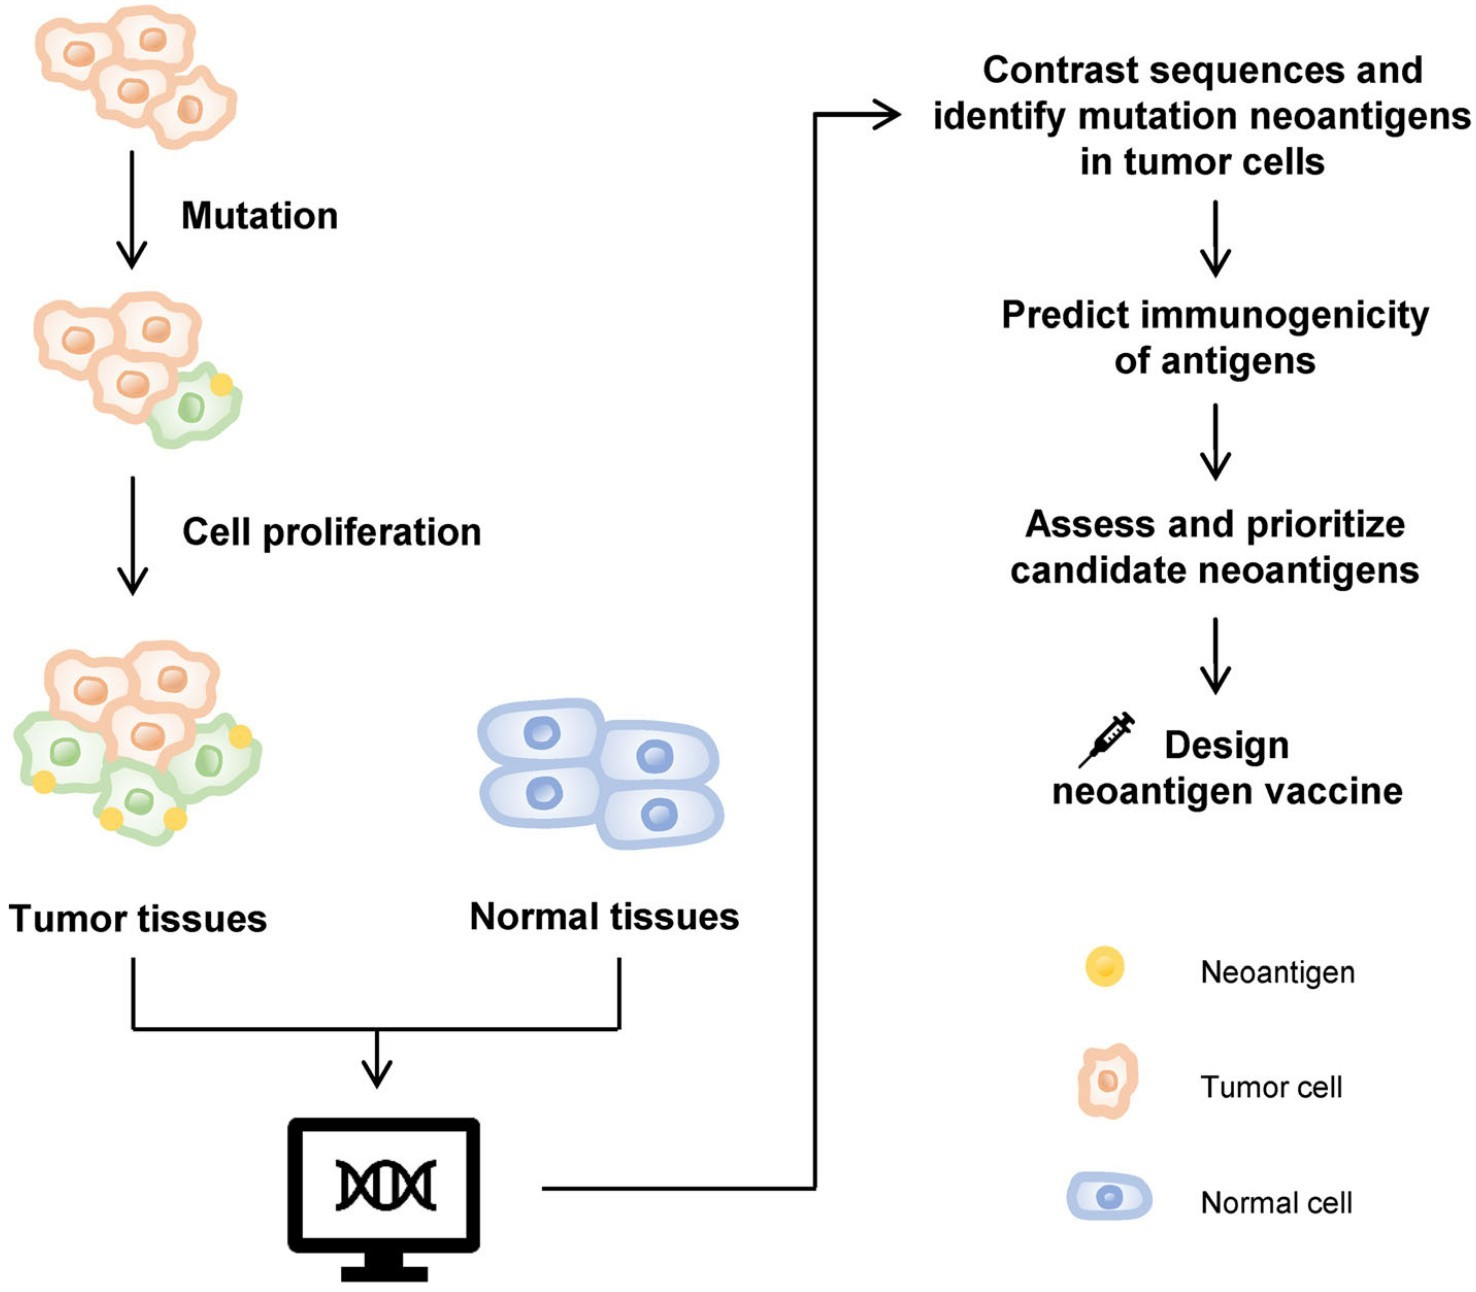
\includegraphics[width=0.7\textwidth]{img/neoantigen/process}	
	\caption{Proceso para la generación de vacunas personalizadas. Fuente: \citep{de2020neoantigen} }
	\label{fig:process}
\end{figure}

Existen herramientas de Software que se basan en la predicción del enlace entre las moléculas Major Histocompatibility Complex (MHC) y péptidos (posibles neo antígenos). La predicción de estos enlaces es importante para determinar qué péptidos pueden representar neo antígenos. Entre las principales propuestas que utilizan Regresión lineal y Redes Neuronales, tenemos: NetMHC4 \citep{stevanovic2017landscape}, NetMHCpan4 \citep{robbins2013mining}, PickPocket \citep{tran2014cancer}, NetMHCcons \citep{castle2012exploiting}, NetMHCIIpan \citep{yadav2014predicting}. También, existen alternativas como NeonMHC \citep{van2013tumor} que utilizan Redes Neuronales Convolucionales. Luego, otras propuestas se basan en la mejorar la predicción de un posible neo antígeno \citep{lu2021deep, hao2021improvement, lang2021neofox, chen2021identification, yang2021deepnetbim, li2021deepimmuno}.  Una desventaja de estos métodos, es referente a la necesidad de contar de antemano con posibles peptidos, esto complica una propuesta \textit{end-to-end} que tome como entrada una secuencia de ADN.\\

Debido a la complejidad del proceso y la gran cantidad de métodos desarrollados, se ha desarrollado software y \textit{pipelines} que pretenden facilitar el uso de estas herramientas. Entre las más recientes tenemos: Somaticseq \citep{fang2015ensemble}, NeoPredPipe \citep{schenck2019neopredpipe}, CloudNeo \citep{bais2017cloudneo}, MuPeXI \citep{bjerregaard2017mupexi}, NeoepitopePred \citep{tran2015immunogenicity}, Neoepiscope \citep{yossef2018enhanced}, pVACtools \citep{hundal2020pvactools}  y NeoFuse \citep{gros2016prospective}. Estas herramientas en su mayoría toman como entrada archivos Variant Calling Files (VCF) y archivos de alineamiento Bam, para la detección de mutaciones (inserciones, eliminaciones y fusión de genes) y posibles neo antígenos. Si bien es cierto, los \textit{pipelines} mencionados anteriormente son propuestas \textit{end-to-end}, el acierto es bajo y son dificiles de desplegar.\\

A pesar de la gran cantidad de métodos y herramientas no existe un método que pueda ser definido como el de mejor desempeño \citep{de2020neoantigen}, incluso a pesar de ya haberse desarrollado algunos \textit{benchmarkings}. Por ejemplo, en el 2015 se desarrolló una comparativa de los métodos SMM, ANN, ARB y NetMHCpan \citep{trolle2015automated}, sin ninguna conclusión sobresaliente. Luego en el 2018 y 2019 se vuelve a intentar realizar otra comparativa \citep{bonsack2019performance, zhao2018systematically}, sin lograr determinar a un método con mayor desempeño. Tambien se han desarrollado \textit{surveys} sobre como los métodos computacionales pueden tener beneficios clínicos \citep{de2020neoantigen} y sus principales desafios \citep{chen2021challenges}. \\

Finalmente, en la Tabla \ref{tab:review}, se presenta un resumen de los métodos basados en \textit{MHC-binding} y \textit{pipelines}. Tambien, indicamos cuales son \textit{open source}.\\

\begin{table}[H]
	\centering
	\caption{Resumen de los métodos de detección de neo antígenos.}
	\label{tab:review}
	\begin{tabular}{llll}
		\hline
		\textbf{Nombre} & \textbf{MHC-binding} & \textbf{Método} & \textbf{Open source} \\ \hline
		NetMHC4         & \checkmark            & ANN             &                      \\
		NetMHCpan4      & \checkmark            & ANN             &                      \\
		PickPocket      & \checkmark            & ANN             &                      \\
		NetMHCcons      & \checkmark            & ANN             &                      \\
		NetMHCIIpan     & \checkmark            & ANN             &                      \\
		NeonMHC         & \checkmark            & CNN             &                      \\
		DeepNetBim      & \checkmark            & Deep learning   & \checkmark            \\
		DeepImmuno      & \checkmark            & CNN             &                      \\
		NeoPredPipe     &                      & pipeline        & \checkmark            \\
		CloudNeo        &                      & pipeline        &                      \\
		MuPeXI          &                      & pipeline        &                      \\
		NeoepitopePred  &                      & pipeline        &                      \\
		Neoepiscope     &                      & pipeline        &                      \\
		pVACtools       &                      & pipeline        & \checkmark            \\
		NeoFuse         &                      & pipeline        & \checkmark    \\   \hline    
	\end{tabular}
\end{table}
